\documentclass{beamer}

\usepackage[size=a4,orientation=landscape,scale=1.5]{beamerposter}
\usetheme{LLT-poster}
\usecolortheme{Entrepreneur}

\usepackage[utf8]{inputenc}
\usepackage[T1]{fontenc}
\usepackage{libertine}
\usepackage[scaled=0.92]{inconsolata}
\usepackage[libertine]{newtxmath}
\usepackage{wrapfig}
\usepackage{mathtools}
\usepackage{calc}
\usepackage{mwe}

\author[Advisor: Ing. Matej Lexa, Ph.D.]{Miroslav Cupak}
\title{Beacon Network: A System for Global Genomic Data Sharing}
\institute{Faculty of Informatics, Masaryk University, Brno, Czech Republic}

\footimage{
\includegraphics[width=1.4cm]{img/fi-logo.pdf}}

\begin{document}
\begin{frame}[fragile]

\begin{columns}[T]
\begin{column}{.32\textwidth}

\begin{block}{Motivation\hfill\raisebox{\heightof{B)}-\height+2pt}{
\includegraphics[height=1em]{img/idea.png}}}
\textit{"The only way to deal with variants of unknown significance is to create a large-scale genomic knowledge network that includes all the genetic variants observed worldwide, and their associated health observations. This requires a global network of shared data. The vast majority of human genetic variants are individually rare but collectively common, so this effort will have health impact on almost everybody."}
\begin{flushright}
David Haussler, Director of UCSC Genomics Institute
\\\footnotesize \url{https://genomics.soe.ucsc.edu/news/article/172}
\end{flushright}
\vspace{-2mm}

\begin{itemize}
\item Genomics is the key to understanding human health.
\item Data generation is exponential.
	\begin{itemize}
	\item Cost of genome sequencing down 1M times during the recent years.
	\begin{center}
	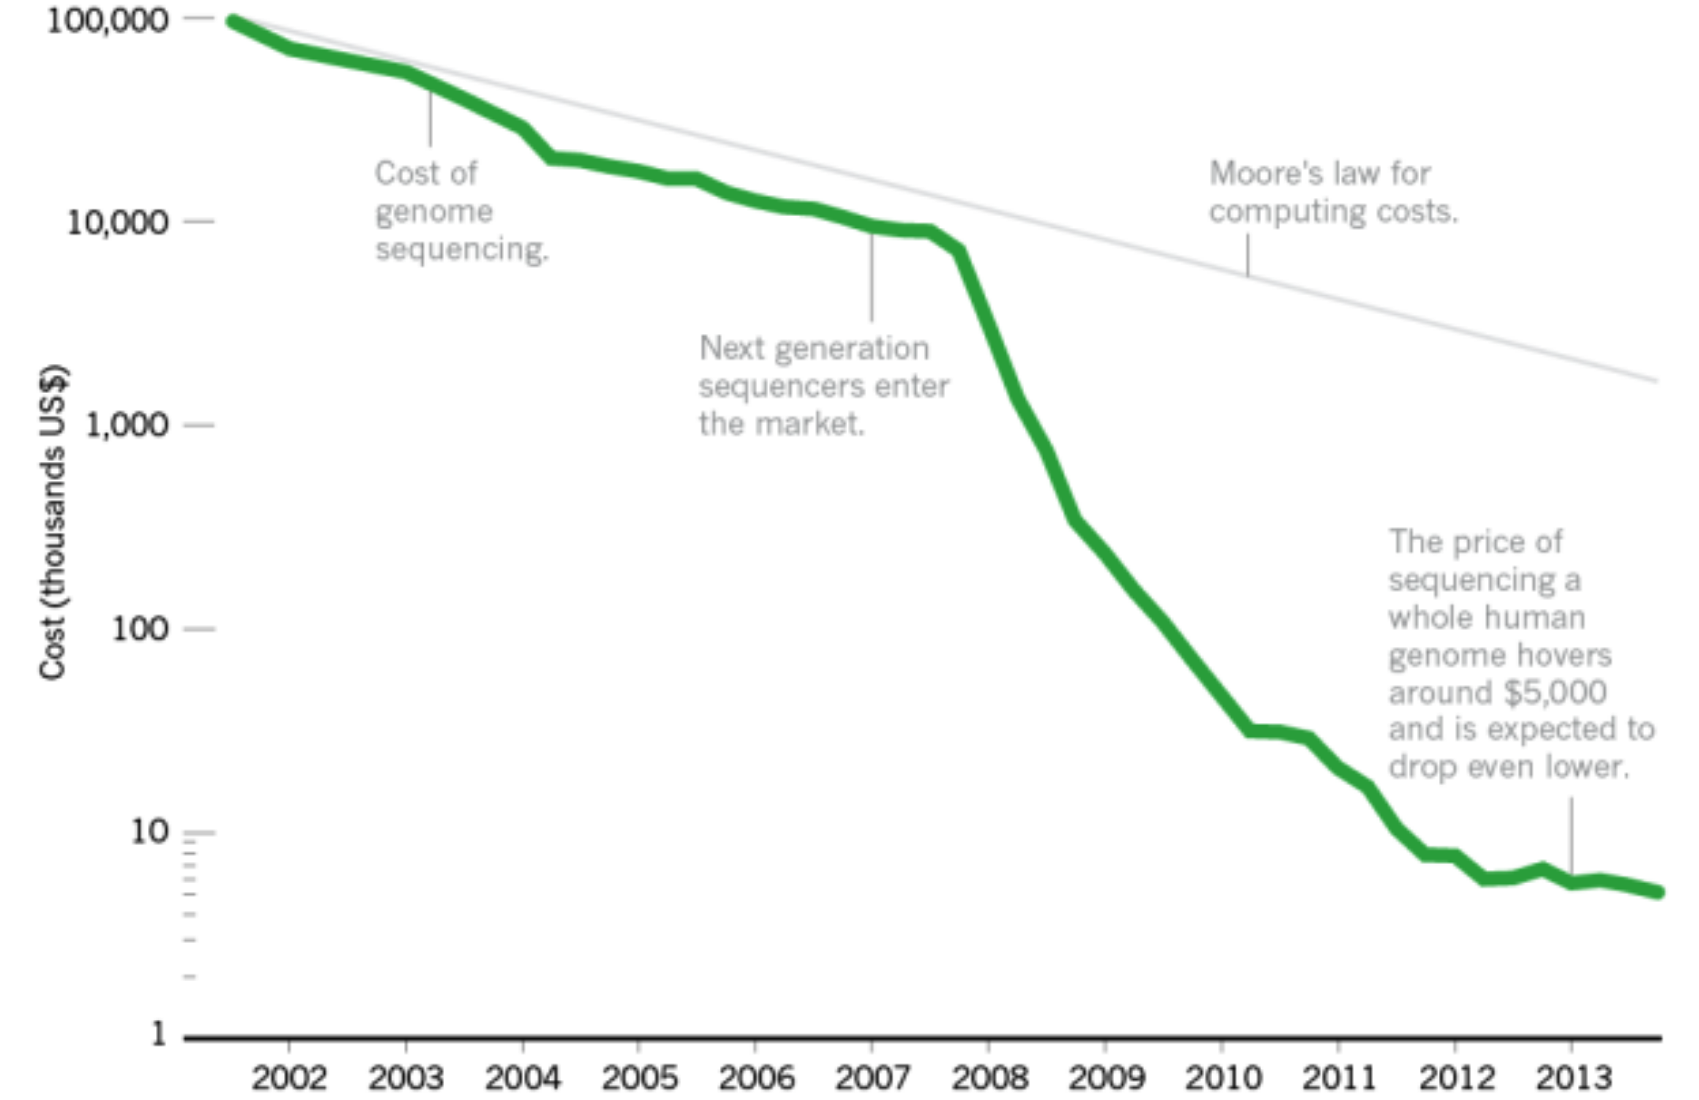
\includegraphics[height=14em,width=\linewidth]{img/sequencing.png}
	\vspace{-2mm}
	\end{center}
	\begin{flushright}
	\footnotesize Hayden, E. C. (2014). Technology: The \$1,000 genome. Nature 507(7492): 294-295.	
	\end{flushright}
	\item \small 100M-2B humans sequenced by 2025 (4-5 orders of magnitude rise).
	\begin{center}
	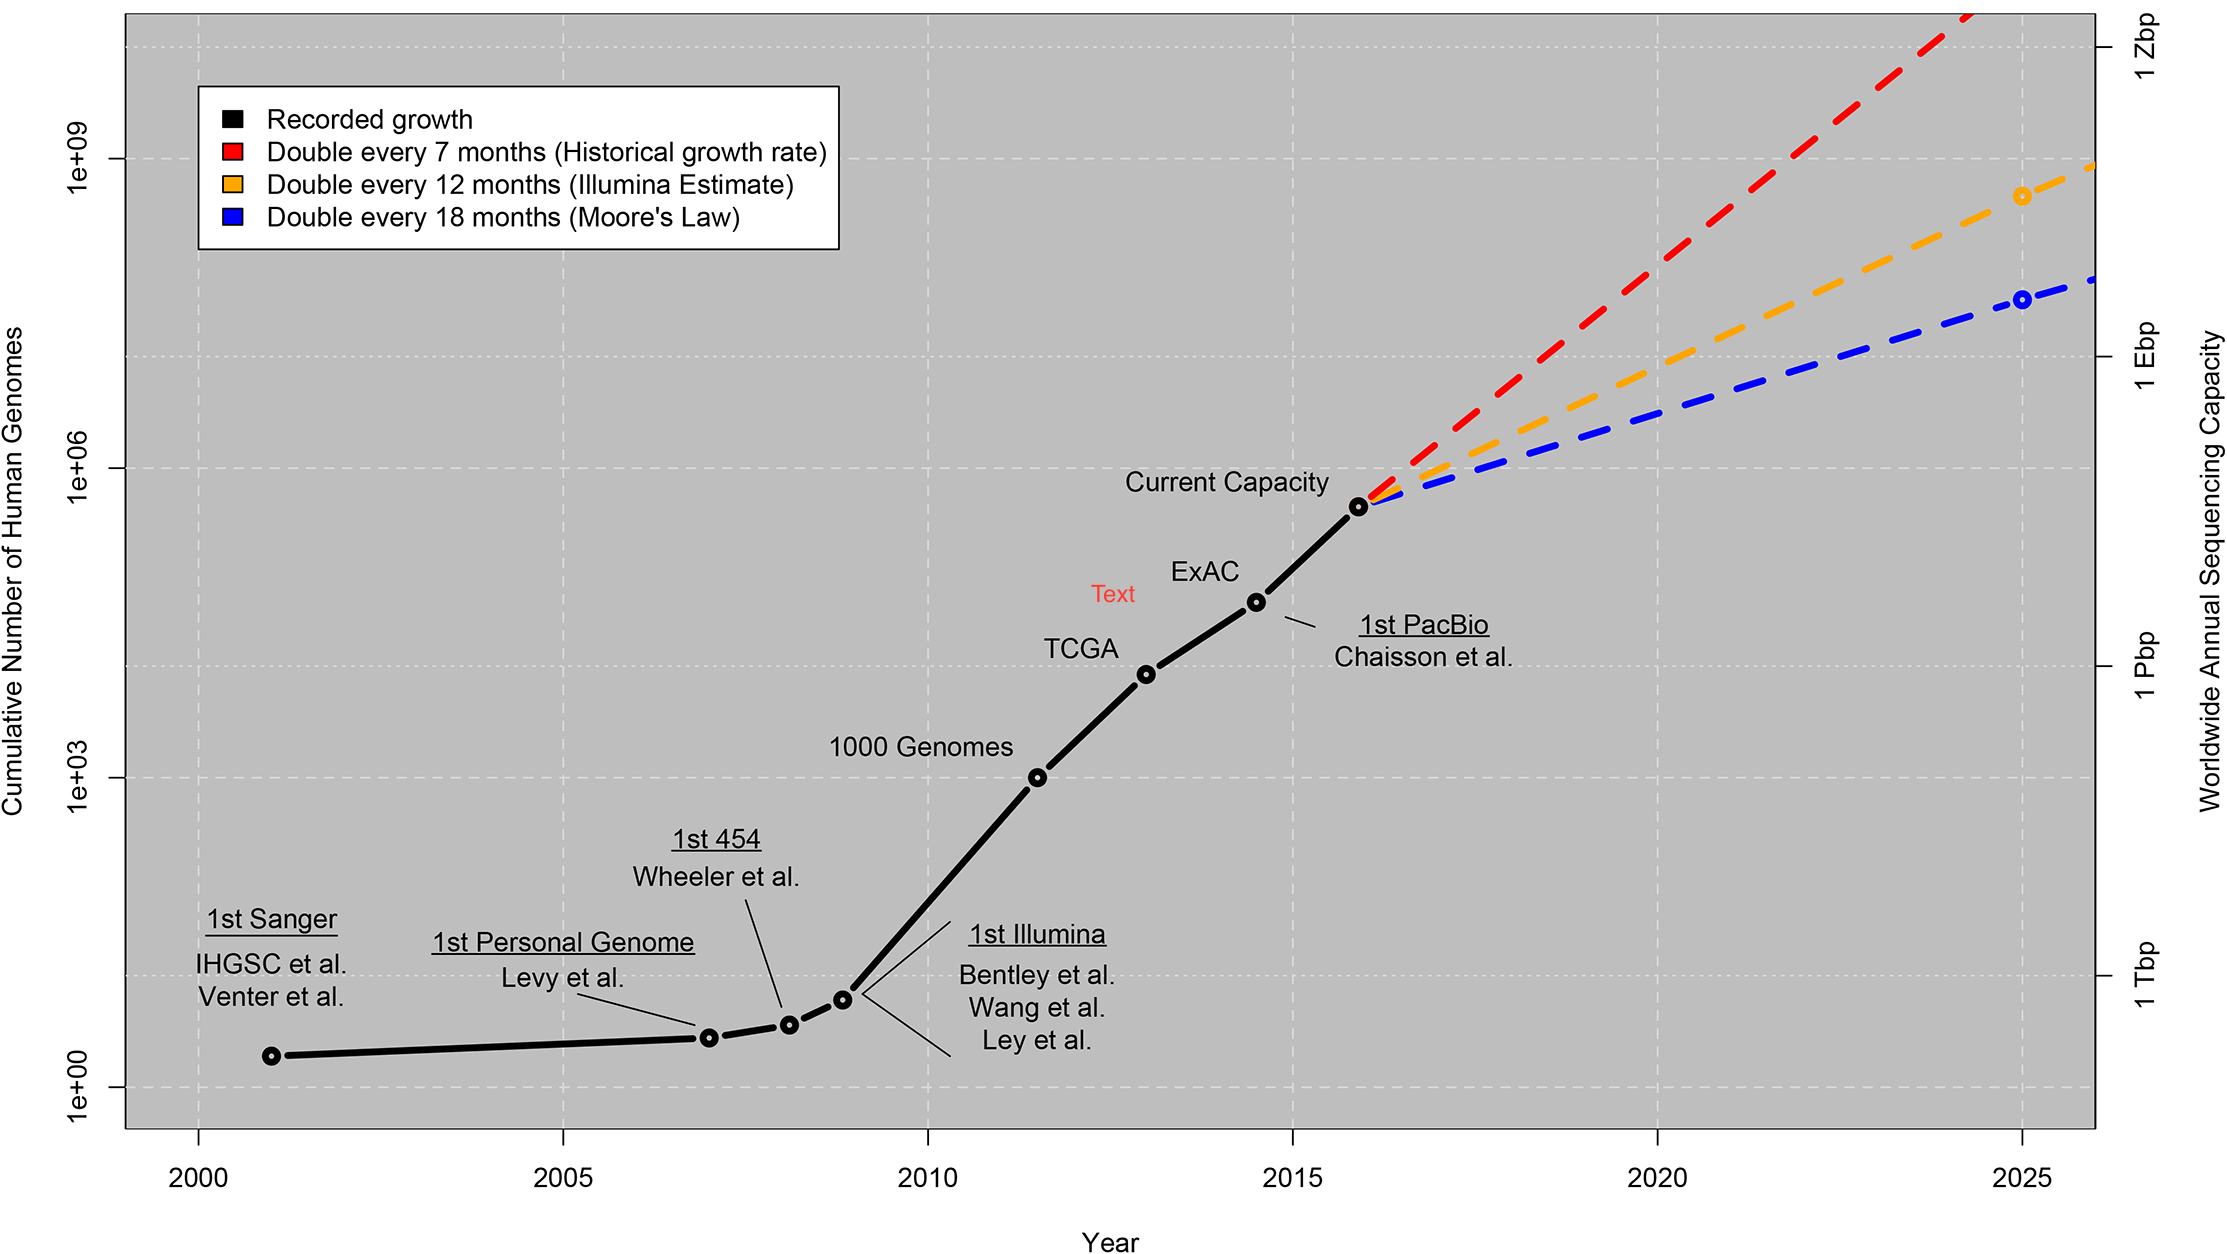
\includegraphics[width=\linewidth]{img/growth.png}
	\vspace{-2mm}
	\end{center}
	\begin{flushright}
	\footnotesize Stephens ZD, Lee SY, Faghri F, Campbell RH, Zhai C, Efron MJ, et al. (2015). Big Data: Astronomical or Genomical? PLoS Biol 13(7): e1002195.
	\end{flushright}
	\vspace{-2mm}
	\end{itemize}
\item Aggregating data in a centralized site is no longer enough.
\item A key obstacle to solving diseases is the difficulty of discovering additional affected families efficiently.
\end{itemize}
\vspace{-1mm}
\end{block}
\end{column}

\begin{column}{.31\textwidth}
\begin{block}{Beacon \hfill\raisebox{\heightof{B)}-\height+2pt}{
\includegraphics[height=1em]{img/beacon.png}}}
\begin{itemize}
\item Web service for genetic data sharing.
\item Receives questions of the form \textit{"Do you have information about this mutation?"}.
\item Responds with \textit{"yes"} or \textit{"no"}, optionally with additional information about the mutation.
\item Initiative of the Global Alliance for Genomics \& Health.
	\begin{itemize}
	\item Coalition of over 400 institutions developing standards for sharing of genomic and clinical data.
	\end{itemize}
\end{itemize}
More information: \url{https://genomicsandhealth.org/work-products-demonstration-projects/beacon-project-0}.
\end{block}

\begin{block}{Beacon Network \hfill\raisebox{\heightof{B)}-\height+2pt}{
\includegraphics[width=1em]{img/ga4gh.png}}}
\begin{itemize}
\item Search engine across the world's public beacons.
\item Answers questions of the form \textit{"Who has information about this mutation?"}.
\item Works by translating genomic queries for each beacon, intelligently distributing the queries through the network, and aggregating the results.
\end{itemize}
\begin{center}
\vspace{-1em}
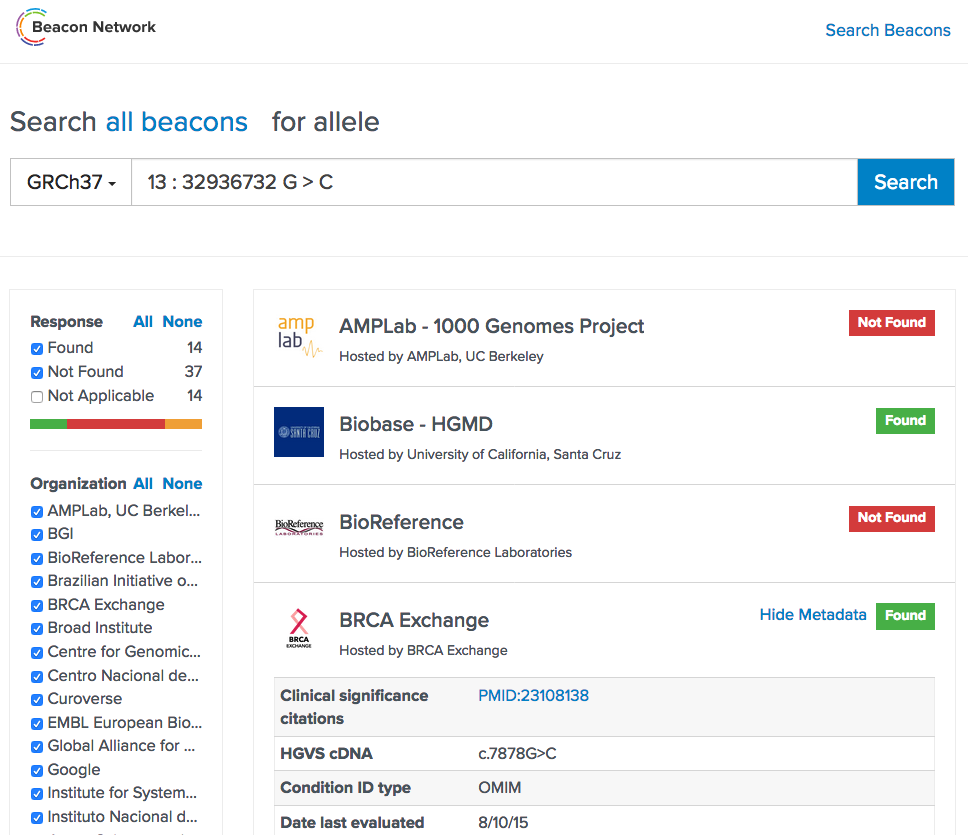
\includegraphics[width=\linewidth]{img/client.png}
\vspace{-1em}
\end{center}
More information: \url{https://beacon-network.org}.
\end{block}
\end{column}

\begin{column}{.35\textwidth}
\begin{block}{Status today\hfill\raisebox{\heightof{B)}-\height+2pt}{
\includegraphics[height=1em]{img/today.png}}}
\begin{itemize}
\item Biggest search and discovery engine of human genomic variation in the world.
\item 25+ of the world's top genomic organizations, 60+ beacons.
\begin{center}
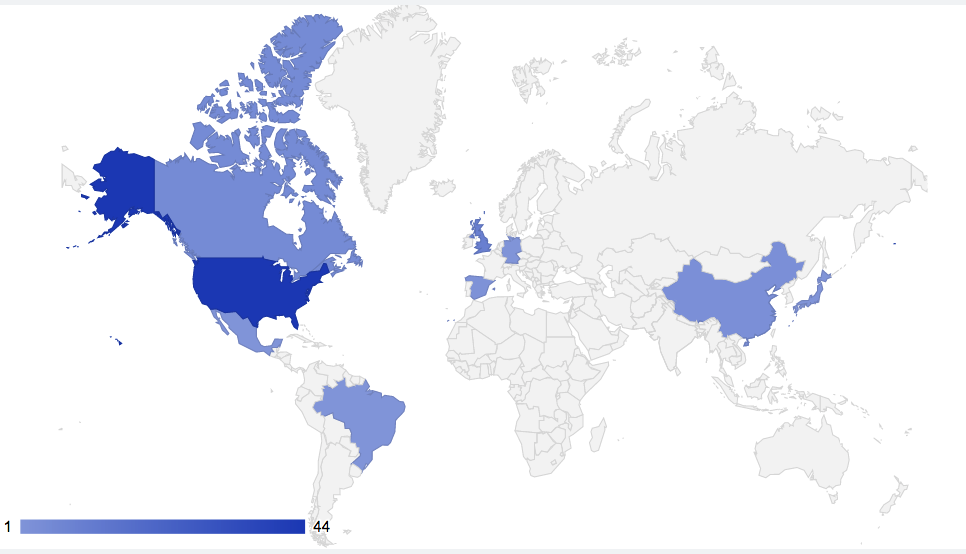
\includegraphics[width=\linewidth]{img/map.png}
\end{center}
\item Served 400K+ genomic queries resulting in 2M+ queries dispatched to the participants of the network.
\begin{center}
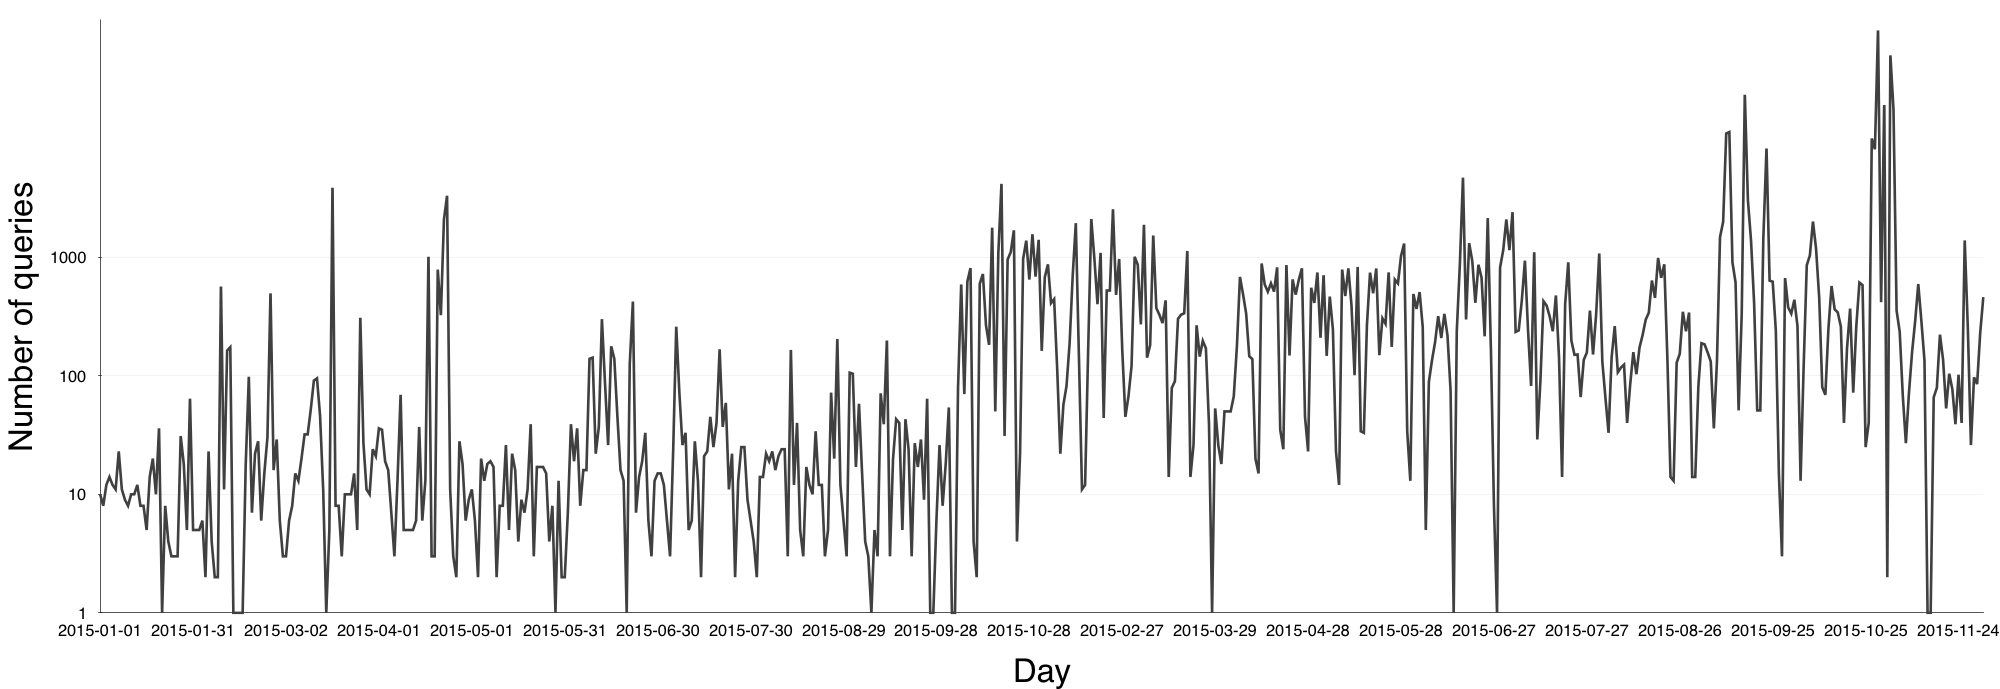
\includegraphics[width=\linewidth]{img/queries.png}
\end{center}
\item Search spanning est. 2M+ samples and 2B+ mutations.
\item 6K+ users from 100+ countries.
\item Queries targeting harmful genetic variations, rare diseases and otherwise interesting or unusual genes and phenotypes.
\item Mentioned in several scientific publications and press articles, presented at major conferences (e.g. ASHG, BioData World).
\item Integrated in commercial products (e.g. DNAstack, Omnicia).
\item Influences standards for how genomic data is shared, drives development of the Beacon API specification.
\item Now REST API, web frontend, command line client, query library, compatible beacon implementations in multiple programming languages, and adapters for various sources of genomic data.
\end{itemize}
\end{block}
\end{column}

\end{columns}
\end{frame}
\end{document}